\section{Finally Big Data}

\subsection{Map Reduce Model}

\textbf{How can I scale the transformations to bilions of rows?}

MapReduce is a programming model proposed in a Google paper (2003)to easier multi-node process parallelization:

\begin{itemize}
	\item Users specify a map function that processes a key/value pair to generate a set of intermediate key/value pairs, and a reduce function that merges all intermediate values associated with the same intermediate key
	\item Programs written in this functional style are automatically parallelized and executed on a large cluster of commodity machines
	\item Inputs and operations over inputs are processed in parallel by different machines using a partitioning function (e.g., hash(key) mod R)
\end{itemize}  

\begin{center}
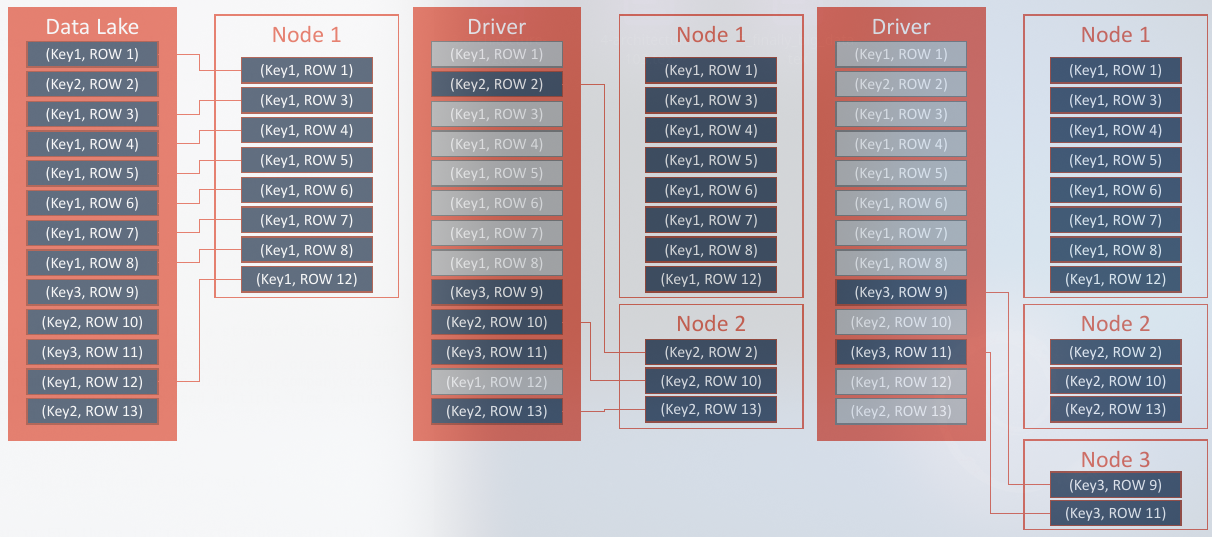
\includegraphics[scale=0.5]{51-map-reduce-model-1}
\end{center}

\begin{center}
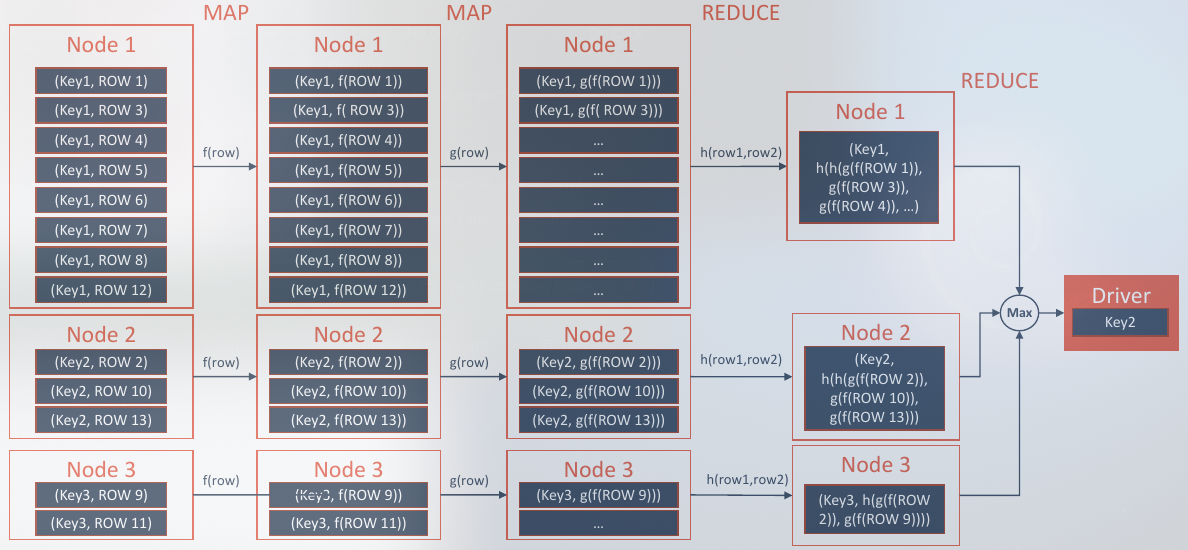
\includegraphics[scale=0.5]{51-map-reduce-model-2}
\end{center}

\subsection{Apache Hadoop}

\textbf{Distributed Parallel Frameworks}

\textbf{How to process data at scale}

\begin{itemize}
	\item Framework of -mostly- \textbf{open source components} built to facilitate the development of multi-node services written in Java
	\item Based on the assumption \textbf{hardware can fail}, several high reliability strategies are used inside Hadoop
	\item Three main components
	- \textbf{STORAGE} - Hadoop Distributed File System Storage (HDFS)
	- \textbf{RESOURCE MANAGEMENT} - Hadoop YARN
	- \textbf{PARALLEL COMPUTATION} - Hadoop MapReduce (implementation of Map Reduce pattern)
	\item Any Hadoop component should be location aware (name of the network switch where each node is) and should share it to the system to distribute data and computation
\end{itemize}

\subsubsection{Apache Architecture}

\begin{center}
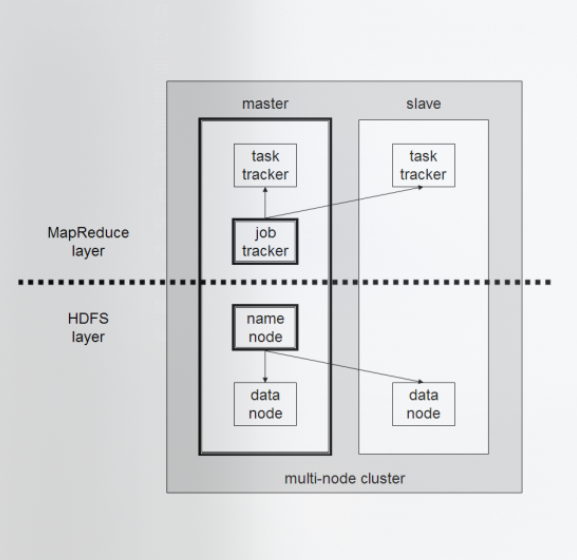
\includegraphics[scale=0.5]{52-hadoop-architecture-1}
\end{center}

\begin{itemize}
	\item \textbf{Job Tracker}
	- service that decide where a given task should be executed (ideally the nodes that have the data, or closer one)
	\item \textbf{Task Tracker}
	- a nde in the cluster that accepts tasks from a JobTracker. It expose a finite number of slots that represents its capability of run parallel tasks. Each task is executed on a spawned JVM. It also sends an heartbeat to the Job Tracker every minute to reassure it is still alive
\end{itemize}

\begin{itemize}
	\item \textbf{NameNode}
	- It keeps the directory tree of all files in the file system, and tracks where across the cluster the file data is kept. It does not store the data of these files itself. It is the Single Point of Failure of an Hadoop application. It routes request between application and DataNode
	\item \textbf{Backup NameNode}
	- Still under development to give to Hadoop High Availability
	\item \textbf{DataNode}
	- Stores data. DataNodes work with each other to replicate data. DataNode with data to process should be deployed on the same machine where TaskTracker is running
\end{itemize}

\begin{itemize}
	\item \textbf{Master Node}
	- Made by a Job Tracker, Task Traker, NameNode, and DataNode
	\item \textbf{Worker Node}
	- Made by a DataNode and TaskTracker
\end{itemize}


\subsubsection{Apache Sequence}

\begin{center}
\includegraphics[scale=0.5]{52-hadoop-architecture-sequence}
\end{center}

\begin{itemize}
	\item Application submits an asyncronous job to the Job Tracker, then it can start polling the Job Tracker for job status
	\item Job Tracker gets data locations in the Name Node registry
	\item Job Tracker identifies the set of Task Trackers with available slots nearest to Data Nodes
	\item The JobTracker submits the work to the chosen Task Trackes
	\item ob Tracker starts to monitor Task Trackers heartbeat: If they do not submit heartbeat signals often enough, it presumes they failed and work is scheduled on a different Task Tracker.
	\item When each Task Tracker completes the task, it notify the Job Tracker the final status. If it failed, the Job Tracker can:
	1. resubmit the job elsewhere
	2. mark that specific record as to-skip
	3. blacklist the task traker as unreliable
\end{itemize}

\textbf{Moving computation is Cheaper than Moving Data}
A computation requested by an application is much more efficient if it is executed near the data it operates on. This is especially true when the size of the data set is huge. This minimizes network congestion and increases the overall throughput of the system. The assumption is that it is often better to migrate the computation closer to where the data is located rather than moving the data to where the application is running. HDFS provides interfaces for applications to move themselves closer to where the data is located.

\subsection{Hadoop Distributed File System Storage HDFS}

\textbf{HDFS is a distributed file syste designed to run on commodity hardware}

\begin{itemize}
	\item HDFS is highlt \textbf{foult-tolerant} and is designed to be deployed on low-cost hardware.
	\item HDFS provides \textbf{high throughput} access to application data and is suitable for applications that have large data sets.
\end{itemize}

\subsection{Hadoop YARN}

\textbf{YARN is based on the idea to split up the functionalities of resource management and job scheduling/monitoring into separate daemons}

\begin{itemize}
	\item Global ResourceManager (RM)
	ultimate authority that arbitrates resources among all the applications in the system
	\item [per-machine] NodeManager
	monitoring machine resource usage and reporting the same to the ResourceManager/Scheduler.
	\item [per-application] ApplicationMaster (AM)
	negotiating resources from the ResourceManager and working with the NodeManager(s) to execute and monitor the tasks.
\end{itemize}

\subsection{Hadoop Map Reduce}

\textbf{Hadoop MapReduce is a framework that implement MapReduce model taking care of scheduling tasks, monitoring them and re-executes the failed tasks.}

\begin{itemize}
	\item It consist of
	- a single master ResourceManager
	- one morker NodeManger per cluster-node
	- one AppMaster per application
	\item The Hadoop job client submits the job and configuration to the ResourceManager which then assumes the responsibility of distributing it to the workers
\end{itemize}

\subsubsection{Apache Sqoop}

Sqoop is a command-line interface application for transferring data between relational databases and Hadoop.

Sqoop supports incremental loads of a single table or a free form SQL query as well as saved jobs which can be run multiple times to import updates made to a database since the last import.

\textbf{Apache Sqoop (and CDC)}

\begin{center}
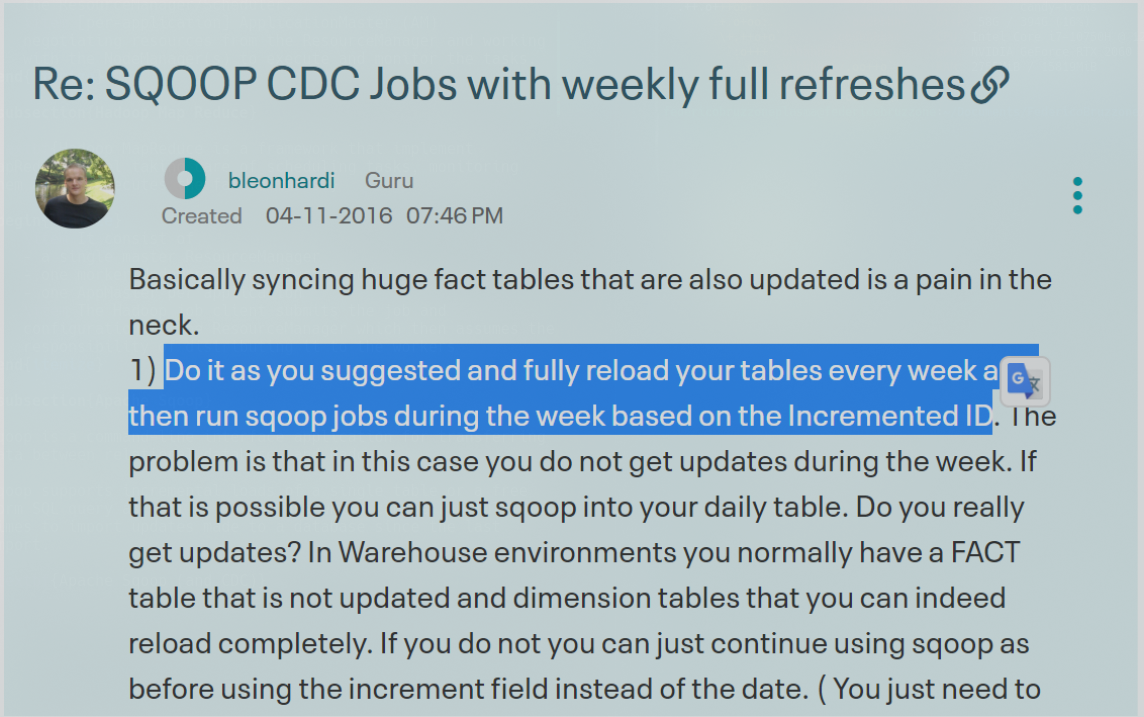
\includegraphics[scale=0.5]{53-apache-sqoop}
\end{center}

\subsubsection{Apache Hive}

Apache Hive is a data warehouse software project built on top of Apache Hadoop for providing data query and analysis.

Hive gives a SQL-like interface and a specific dialect HiveQL that is translated in Hadoop MapReduce jobs to query data.

Hive vs SQL:

Schema on Read         | Schema on Write

More efficient Write   | Less efficient Write

Less efficient queries | More efficient queries

\subsection{Data Lake over HDFS}

\subsubsection{Hadoop Architecture – HDFS}

\begin{center}
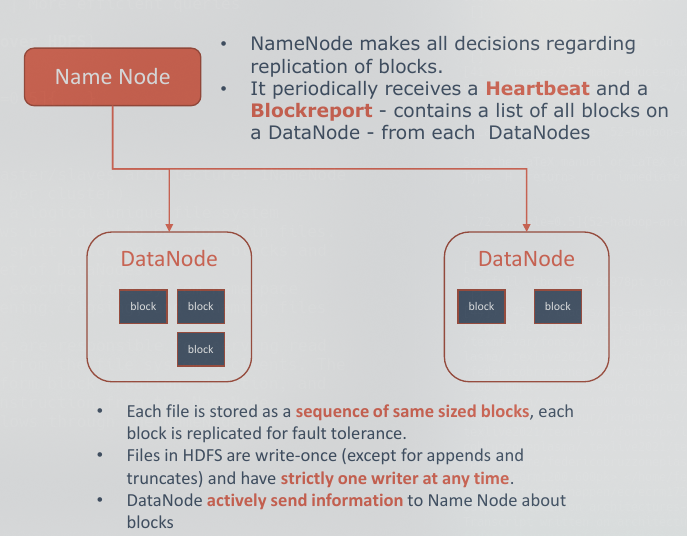
\includegraphics[scale=0.5]{54-hdfs-1}
\end{center}

\begin{itemize}
	\item HDFS has a master/slaves architecture: 1NameNode per n Datanodes (1 per cluster)
	\item HDFS exposes a logical unique file system namespace and allows user data to be stored in files.
	\item Each file is split into one or more blocks and distributed in a set of DataNodes.
	\item The NameNode executes file system namespace operations like opening, closing, and renaming files and directories.
	\item The DataNodes are responsible for serving read and write requests from the file system’s clients. The DataNodes also perform block creation, deletion, and replication upon instruction from the NameNode.
	\item Data never flows through the NameNode.
\end{itemize}

\textbf{HOW CAN WE WRITE WITH THOUSANDS OF SLAVES?}

\subsubsection{Hadoop Architecture – HDFS Replication Policy}

\begin{center}
\includegraphics[scale=0.5]{55-hdfs-2}
\end{center}

\begin{itemize}
	\item The NameNode determines the rack id each DataNode
	\item Placement of replicas are rack-aware to:

	- optimize network bandwidth

	- increase faoult tollerance

	- increase I/O performance
	\item Policy 1 – Replicate the entire rack Placement policy is to replicate the entire rack

	- prevents losing data if an entire rack fails

	- allows routing read requests over different racks optimizing network usage

	- Make easier re-load-balancing on component failure

	- increases the cost of writes because a write needs to transfer blocks to multiple racks.
\end{itemize}

\begin{center}
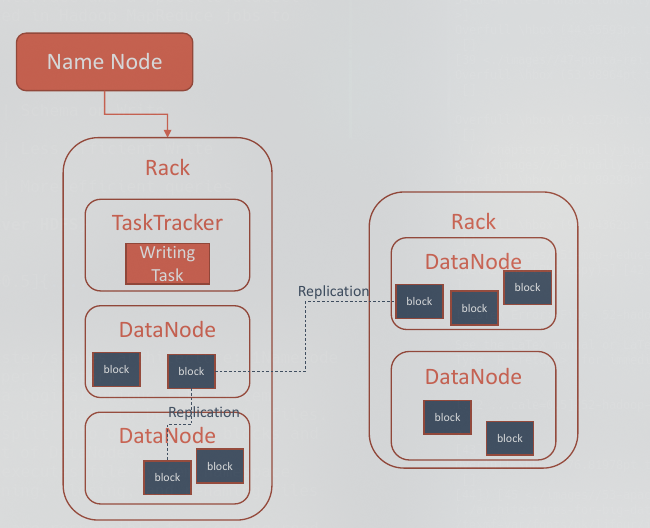
\includegraphics[scale=0.5]{56-hdfs-3}
\end{center}

\begin{itemize}
	\item Policy 2 – Two rack factor 3 replication Placement policy is to put one replica on a DataNode where the writer task is, another replica on a node in a different (remote) rack, and the last on a different node in the same remote rack.

	- Improved write performance: cuts the interrack write traffic

	- Sub-optimal reading: a block is placed in only two unique racks rather than three.

	- Sub-optimal file distribution:

		- one third of replicas are on one node,

		- two thirds of replicas are on one rack,

		- and the other third are evenly distributed across the remaining racks
\end{itemize}

